\section{Time efficiency analysis}
\label{appendix:time_efficiency}

\subsection{Computational complexity compare to standard bilevel optimization}  
We compare the per‐iteration cost of our single‐epoch inner loop against the full‐training inner loop used in bilevel-CADS, and then account for the one-time cost of fitting the loss estimator $l(|\bm m|)$.

Let
\begin{itemize}
  \item $|\mathcal D|$ be the size of the training set,  
  \item $T_{\mathrm{ep}}=O(|\mathcal D|)$ the cost of one full epoch (one forward+backward pass),  
  \item $N$ the number of epochs used by bilevel-CADS in its inner optimizer,  
  \item $K$ the number of subsets sampled per outer iteration,  
  \item $|\bm m|$ the average subset size,  
  \item $M$ the total number of outer iterations in a run.
\end{itemize}

\paragraph{Bilevel-CADS inner solve (per outer step)}  
\[
\mathrm{Cost}_{\rm bilevel}
\;=\;
K \times N \times T_{\mathrm{ep}}
\;=\;
O\bigl(KN\,|\mathcal D|\bigr).
\]

\paragraph{Our CADS-E/S inner loop (per outer step, ignoring estimator)}  
\[
\mathrm{Cost}_{\rm CADS}^{\rm base}
\;=\;
K \times T_{\mathrm{ep}}
\;=\;
O\bigl(K|\mathcal D|\bigr).
\]

\paragraph{Estimator fitting overhead}  
To fit the mapping $l(|\bm m|)$ we train 8 models for $N$ epochs each (As detailed in ~\ref{appendix:gaussian}), incurring a one‐time cost  
\[
\mathrm{Cost}_{\rm est}
\;=\;
8 \times N \times T_{\mathrm{ep}}.
\]
Amortized over $M$ outer steps, this adds  
\[
\frac{\mathrm{Cost}_{\rm est}}{M}
\;=\;
\frac{8\,N\,T_{\mathrm{ep}}}{M}
\]
to each iteration.

\paragraph{Total CADS cost (amortized)}  
\[
\mathrm{Cost}_{\rm CADS}
\;=\;
K\times T_{\mathrm{ep}}
\;+\;
\frac{8\,N\,T_{\mathrm{ep}}}{M}
\;=\;
T_{\mathrm{ep}}\Bigl(K + \tfrac{8\,N}{M}\Bigr).
\]

\paragraph{Speed-up factor}  
\[
\frac{\mathrm{Cost}_{\rm bilevel}}{\mathrm{Cost}_{\rm CADS}}
\;=\;
\frac{K\,N\,T_{\mathrm{ep}}}{T_{\mathrm{ep}}\bigl(K + \tfrac{8\,N}{M}\bigr)}
\;=\;
\frac{K\,N}{K + 8\,N/M}.
\]
In our experiments \(K = 5\) and \(M = 100\), giving
\[
\frac{\mathrm{Cost}_{\rm bilevel}}{\mathrm{Cost}_{\rm CADS}}
\;=\;
\frac{1}{1/N + 0.016}.
\]
In practice, larger $N$ yields an even greater speed-up.

\subsection{Empirical Validation}  

We measure end-to-end wall-clock time of bilevel-CADS and CADS-E on MNIST as a function of compute budget $C$ (total epochs).  We sweep $C$ over $\{5,50,100,200,500,1000,2000,5000\}$ and record the runtime of each method under identical hardware. Figure~\ref{fig:time_efficiency_empirical} confirms a roughly linear scaling for both methods, with CADS-E exhibiting a much smaller slope.


\subsection{Analysis of Selection Algorithm Runtime}
\label{appendix:runtime_analysis}

A potential concern regarding our method is that the runtime of the selection algorithm may scale with the number of sampled subsets (\(K\)), which could offset the computational efficiency gains. We address this concern by highlighting several key aspects of our approach.

\paragraph{Minimal Sampling for Practical Implementation}
Our policy gradient approach for coreset selection requires only a small number of samples (\(K\)) to ensure training stability. For instance, the comparable PBCS method \cite{ds_bi_zhou2022probabilistic} utilizes \(K=1\) for all its experiments. Our results show that using \(K=2\) is sufficient to achieve strong performance while maintaining high computational efficiency. In cases where smaller \(K\) values might lead to higher gradient variance (e.g., in more complex problems), this can be mitigated using established variance reduction techniques. A common approach is to use a self-critical baseline, which adjusts the reward signal as follows:
\begin{equation}
\label{eq:variance_reduction}
\tilde{\mathcal{L}}(S_i) = \mathcal{L}(S_i) - \frac{1}{K} \sum_{j=1}^{K} \mathcal{L}(S_j).
\end{equation}

\paragraph{Amortized Cost of Coreset Selection}
It is important to emphasize that the core contribution of this work is the introduction of computational budget constraints into the coreset selection process, rather than optimizing the selection runtime itself. Once generated, a coreset is a reusable asset that can be applied across various training scenarios, different model architectures, and subsequent experiments. Consequently, the initial computational investment in the selection process is amortized over these multiple uses. This makes the selection efficiency a secondary consideration compared to the quality and utility of the resulting budget-constrained coreset.


\begin{figure}[!htbp]  
  \centering  
  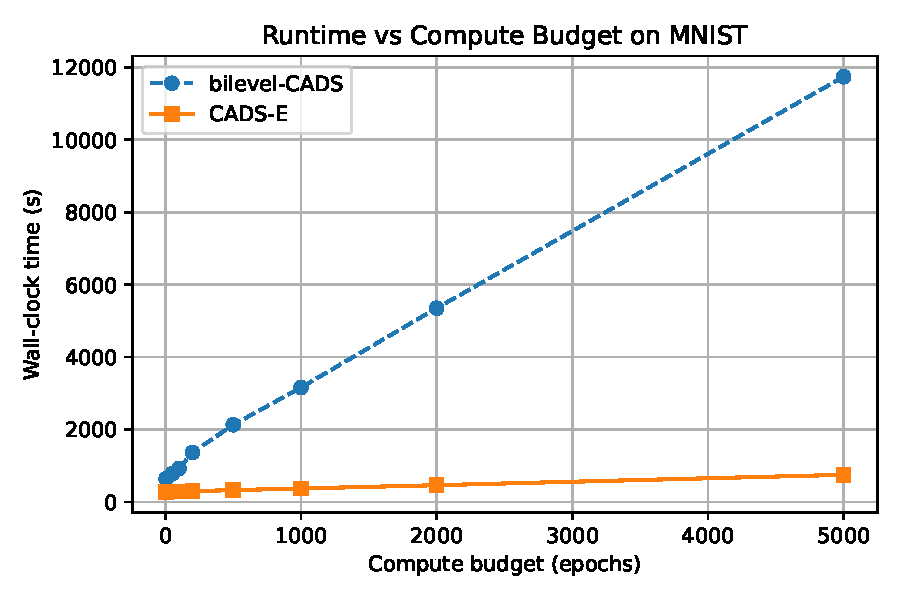
\includegraphics[width=0.6\textwidth]{pics/runtime_vs_budget.pdf}  
  \caption{Wall-clock runtime vs.\ compute budget $C$ for bilevel-CADS (dashed) and CADS-E (solid), MNIST.}  
  \label{fig:time_efficiency_empirical}  
\end{figure}  

